\documentclass[a4paper]{deedy-resume} % Use US Letter paper, change to a4paper for A4 

\begin{document}

%----------------------------------------------------------------------------------------
%	TITLE SECTION
%----------------------------------------------------------------------------------------

\lastupdated % Print the Last Updated text at the top right

\namesection{Stefano}{Forti}{ % Your name
\urlstyle{same}\url{http://stefanoforti.altervista.org} \\ % Your website, LinkedIn profile or other web address
\href{mailto:stefano.forti92@gmail.com}{stefano.forti92@gmail.com} | 333 27 18 311 % Your contact information
}

%----------------------------------------------------------------------------------------
%	LEFT COLUMN
%----------------------------------------------------------------------------------------

\begin{minipage}[t]{0.33\textwidth} % The left column takes up 33% of the text width of the page

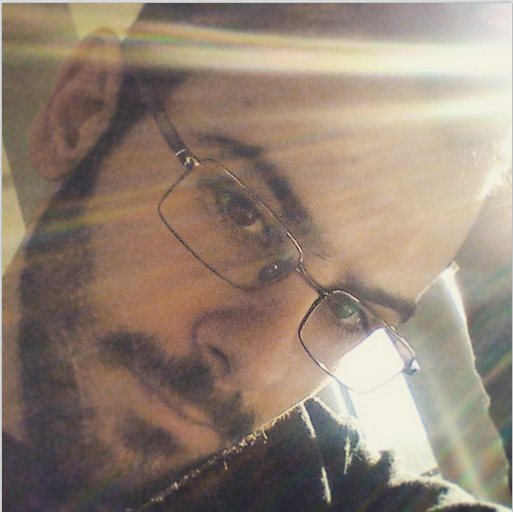
\includegraphics[width=0.5\textwidth]{photo.png}

%------------------------------------------------
% Education
%------------------------------------------------

\section{Educazione} 

\subsection{SSSUP Sant'Anna \& \\Università di Pisa}

\descript{Laurea Magistrale in Informatica e Networking}
\location{Previsto 2016 | Pisa \\ Media: 28}

\sectionspace % Some whitespace after the section

\subsection{Università di Pisa}

\descript{Laurea Triennale in Informatica}
\location{Settembre 2011 - Luglio 2014 | Pisa}
\location{110 e lode}

\sectionspace % Some whitespace after the section

%------------------------------------------------

\subsection{Liceo Scientifico U. Dini}

\descript{Maturità Scientifica PNI}
\location{Settembre 2006 - Luglio 2011 | Pisa}
\location{100 e lode}

\sectionspace % Some whitespace after the section

%------------------------------------------------
% Coursework
%------------------------------------------------

\section{Lingue}

\subsection{Italiano}
\location{Madrelingua}

\subsection{Inglese, Francese}
\location{C1-C2}


\subsection{Cinese}
\location{A1}

\sectionspace % Some whitespace after the section

%------------------------------------------------
% Skills
%------------------------------------------------

\section{Competenze}

Java \textbullet{} Teamwork \textbullet{} \\Parlare in pubblico \textbullet{} Lingue Straniere\textbullet{}\\
Team Leadership\textbullet{} Linguaggi di Programmazione \textbullet{} Scrittura \textbullet{} Videoediting \textbullet{} \LaTeX\ \\ 

\sectionspace % Some whitespace after the section

%------------------------------------------------
% Links
%------------------------------------------------

\section{Links} 

LinkedIn:// \href{https://it.linkedin.com/pub/stefano-forti/89/5a6/348}{\bf stefanoforti} \\
YouTube:// \href{https://www.youtube.com/user/tetus1992/videos}{\bf stefanoforti92} \\
Github:// \href{https://github.com/teto1992/}{\bf teto1992} \\

\sectionspace % Some whitespace after the section

%----------------------------------------------------------------------------------------

\end{minipage} % The end of the left column
\hfill
%
%----------------------------------------------------------------------------------------
%	RIGHT COLUMN
%----------------------------------------------------------------------------------------
%
\begin{minipage}[t]{0.66\textwidth} % The right column takes up 66% of the text width of the page

%------------------------------------------------
% Experience
%------------------------------------------------

\section{Esperienza}

%------------------------------------------------

\runsubsection{\href{http://web.xpreso.com/}{Xpreso}}
\descript{| Consulente Tecnico}

\location{Gennaio 2014 - Giugno 2014 | Dublino, EIRE}
\vspace{\topsep} % Hacky fix for awkward extra vertical space
\begin{tightitemize}
\item collaborazione col team di sviluppo della \textit{start-up}
\item tesi di laurea triennale sulle tecniche di \textit{geocoding}
\end{tightitemize}

\sectionspace % Some whitespace after the section

%------------------------------------------------

\runsubsection{\href{http://www.inlistaperpisa.it/}{In Lista per Pisa}}
\descript{| Candidato}

\location{Gennaio 2013 - Giugno 2013 | Pisa}
\begin{tightitemize}
\item coordinamento del gruppo giovani, stesura e promozione del programma
\item eletto nel CTP 5: mi occupo di cultura, comunicazione e sport
\end{tightitemize}

\sectionspace % Some whitespace after the section

%------------------------------------------------

\runsubsection{la Nazione/l'Ulisse}
\descript{| Coordinatore}

\location{Gennaio 2012 - Maggio 2012 | Pisa}
\begin{tightitemize}
\item ideazione del ciclo di interviste \href{http://www.localistorici.it/it/News/view/slug/all-ussero-tornano-gli-incontri-degli-studenti}{\textit{Un buon tè per pensare...}} in collaborazione coi Locali Storici d'Italia
\item collaborazione con l'Ulisse e \href{http://rassegnastampa.unipi.it/rassegna/archivio/2012/02/21SIG2034.PDF}{la Nazione - Pisa}
\end{tightitemize}

\sectionspace % Some whitespace after the section

%------------------------------------------------

\runsubsection{\href{http://lulisse.altervista.org/}{l'Ulisse - il periodico del Dini}}
\descript{| Vicedirettore}

\location{Settembre 2008 - Settembre 2011 | Pisa}
\begin{tightitemize}
\item direzione del comitato di redazione, organizzazione di eventi culturali e interviste pubbliche
\item scrittura di articoli e comunicati stampa
\end{tightitemize}

\sectionspace % Some whitespace after the section

%------------------------------------------------

\runsubsection{\href{http://www.faretv.net/}{FareTV}}
\descript{| Presentatore}

\location{Settembre 2010 - Giugno 2011 | Pisa}
\begin{tightitemize}
\item ideazione e conduzione del ciclo di interviste \href{http://www.faretv.net/home/trasmissioni/4-incontri-per-fare-gli-italiani}{\textit{fare gli italiani...}}
\end{tightitemize}

\sectionspace % Some whitespace after the section

%------------------------------------------------

\runsubsection{\href{http://temi.repubblica.it/limes/}{liMes}}
\descript{| Responsabile Studenti}

\location{Gennaio 2009 - Giugno 2010 | Pisa}
\begin{tightitemize}
\item coordinamento dei cento studenti coinvolti in uno studio geopolitico sulla città di Pisa
\item pubblicazione su liMes 3/2010 di \href{http://temi.repubblica.it/limes/la-russia-sovrana/15767}{\textit{Anatomia Geopolitica di Pisa}}
\end{tightitemize}

\sectionspace % Some whitespace after the section

%------------------------------------------------

\runsubsection{\href{http://www.cspdiciolo.it/}{Club Scherma Pisa A. Di Ciolo}}
\descript{| Addetto Stampa}

\location{Gennaio 2009 - Dicembre 2010| Pisa}
\begin{tightitemize}
\item pubbliche relazioni con la stampa locale e gestione sito web
\end{tightitemize}

\sectionspace % Some whitespace after the section

%------------------------------------------------

\runsubsection{\href{http://www.ducati.com/index.do}{Ducati Motor Holding}}
\descript{| Stage}

\location{Marzo 2010 | Borgo Panigale (BO)}
\begin{tightitemize}
\item settori: creatività, marketing, corse
\end{tightitemize}

\sectionspace % Some whitespace after the section

%------------------------------------------------
% Awards
%------------------------------------------------

\section{Awards} 

\begin{tabular}{rll}
2013	 & membro della squadra 62/92 per \href{http://www.nwerc.eu/}{NWERC'13}\\
2013	 & membro della squadra seconda classificata per \href{http://www.cs.nott.ac.uk/~mlw/ukiepc/}{UKIEPC'13} in Irlanda\\
2011	 & premio di studio Alberto Ottolenghi del\href{http://www.maestrilavoro.it/index/elenco_consolati/it-toscana-pisa.html}{Consolato dei Maestri del Lavoro}\\
2011	 & \href{http://www.indire.it/eccellenze/}{Albo Nazionale delle Eccellenze MIUR}\\
2010	 & vincitore del premio di scrittura teatrale nell'ambito di EroeMaiCantato IV\\
\end{tabular}

\sectionspace % Some whitespace after the section

%----------------------------------------------------------------------------------------

\end{minipage} % The end of the right column

%----------------------------------------------------------------------------------------
%	SECOND PAGE (EXAMPLE)
%----------------------------------------------------------------------------------------

%\newpage % Start a new page

%\begin{minipage}[t]{0.33\textwidth} % The left column takes up 33% of the text width of the page

%\section{Example Section}

%\end{minipage} % The end of the left column
%\hfill
%\begin{minipage}[t]{0.66\textwidth} % The right column takes up 66% of the text width of the page

%\section{Example Section 2}

%\end{minipage} % The end of the right column

%----------------------------------------------------------------------------------------

\end{document}